% Template; to be used with:
%          spconf.sty  - ICASSP/ICIP LaTeX style file, and
%          IEEEbib.bst - IEEE bibliography style file.
% --------------------------------------------------------------------------
\documentclass{article}
\usepackage{spconf,amsmath,graphicx}

% Example definitions.
% --------------------
\def\x{{\mathbf x}}
\def\L{{\cal L}}

% Title.
% ------
\title{Graduate Certificate Intelligent Sensing Systems Practice Module Report - Early Detection and Diagnostic of Prostate cancer​ (High Quality Segmentation)}
%
% Single address.
% ---------------
\name{Zhang Yu (A0213498X),  Natarajan Anandan(A0213514U) }
\address{Group 9, Institute of Systems Science, National University of Singapore, Singapore 119615}

\begin{document}
%\ninept
%
\maketitle
%

\begin{abstract}

Cancer detection has always been a major issue for the pathologists and medical practitioners for diagnosis and treatment planning. The manual identification of cancer from microscopic biopsy images is subjective in nature and may vary from expert to expert depending on their expertise and other factors which include lack of specific and accurate quantitative measures to classify the biopsy images as normal or cancerous one. The automated identification of cancerous cells from microscopic biopsy images helps in alleviating. As part of this practice module project, we aim to provide a system to automate the identification of the cancerous cells from microscopic biopsy images which can be used by doctors and pathologist for early detection and treatment. We have proposed a method of segmentation and classification technique based on the features and utilized Unet model for segmentation.

Video: https://youtu.be/F6nC36dUT6I

\end{abstract}
%
\begin{keywords}
early detection, identification, segmentation technique 
\end{keywords}
%
\section{Introduction}
\label{sec:intro}

Cancer detection has always been a major issue for the pathologists and medical practitioners for diagnosis and treatment planning. The manual identification of cancer from microscopic biopsy images is subjective in nature and may vary from expert to expert depending on their expertise and other factors which include lack of specific and accurate quantitative measures to classify the biopsy images as normal or cancerous one. For the detection and diagnosis of cancer from microscopic biopsy images, the histo, pathologists normally look at the specific features in the cells and tissue structures. The various common features used for the detection and diagnosis of cancer from the microscopic biopsy images include shape and size of cells, shape and size of cell nucleus, and distribution of the cells.

Prostate cancer is also given a grade called a Gleason score. This score is based on how much the cancer looks like healthy tissue when viewed under a microscope. Less aggressive tumours generally look more like healthy tissue. Tumours that are more aggressive are likely to grow and spread to other parts of the body. They look less like healthy tissue. The Gleason scoring system is the most common prostate cancer grading system used. The pathologist looks at how the cancer cells are arranged in the prostate and assigns a score on a scale of 3 to 5 from 2 different locations. Cancer cells that look like healthy cells receive a low score. Cancer cells that look less like healthy cells or look more aggressive receive a higher score. To assign the numbers, the pathologist determines the main pattern of cell growth, which is the area where the cancer is most obvious, and then looks for another area of growth. The doctor then gives each area a score from 3 to 5. The scores are added together to come up with an overall score between 6 and 10. Gleason scores of 5 or lower are not used. \textbf{The lowest Gleason score is 6, which is a low-grade cancer. A Gleason score of 7 is a medium-grade cancer, and a score of 8, 9, or 10 is a high-grade cancer.} A lower-grade cancer grows more slowly and is less likely to spread than a high-grade cancer.
Here is the current manual process.

\begin{figure}[tbh]
    \centerline{\begin{tabular}{cc|c}
        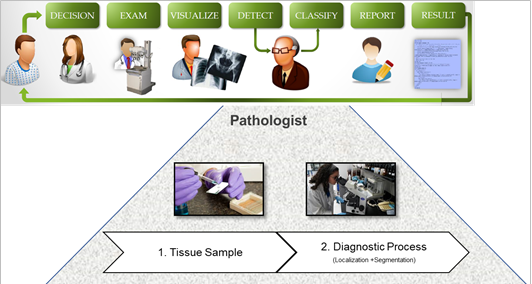
\includegraphics[width=8cm]{current_process1.png}
      \\     \end{tabular}}
    \caption{Current Manual Process.\label{figure1}}
\end{figure}

Challenges with the current process are as follows : 

\begin{figure}[tbh]
    \centerline{\begin{tabular}{cc|c}
        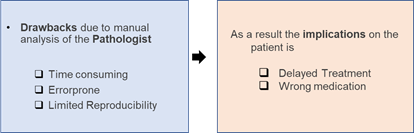
\includegraphics[width=5cm]{current_process_challenge.png}
      \\

    \end{tabular}}
    \caption{Challenges in the Current Manual Process.\label{figure2}}
\end{figure}
Our team had to understand the medical area of cancer and how it is graded. We also went through several papers to know the current areas of research both in the field of automated cancer identification and chemical processing of the tissue samples for better determination of the cancer cells.
We have developed and trained the model,
\begin{enumerate}
\item The\textbf{ input is the image} of the cancerous cell for pathologist to upload. 
\item For training purposes, we have created several samples from the training data available by different augmentation methods.
\item Built the segmentation model and currently performing training to improve the dice coefficient results.
\item The \textbf{output is the image of the segmentation}, shown in the user interface as an image adjacent to the input. 
\end{enumerate}


\section{Literature review}
	Having defined the business problem, our group’s aim is to a novel approach to provide High Quality Segmentation proving extremely helpful in clinical practice for Early Detection and Diagnostic of Prostate cancer. 

To develop a model to classify and segmentation, Our team had to understand the medical are of cancer and how it is graded. We also went through several papers to know the current areas of research both in the field of automated cancer identification and chemical processing of the tissue samples for better determination of the cancer cells. \cite{{NBCI:AIPC}\cite{QUANTIB:AIPC}

The first step is usually a visit to the general practitioner, for example because the patient suffers from pain during urination or from frequent urges to urinate. The GP refers the man to a urologist who starts the hospital-based diagnosis trajectory, including measuring prostate-specific antigen (PSA) levels, increasingly including an MRI exam, and pathology testing. After prostate cancer has been diagnosed, a treatment plan is made. This can be a more direct approach, usually radiation therapy or surgery), or a watchful approach, the active surveillance pathway.\cite{INTEL:DL}

Deep learning methods\cite{NATURE:DCN} have shown promising results in a variety of computer vision tasks such as segmentation, classification, and object-detection. These methods consist of convolution layers that are able to extract different features from low-level local features to high-level global features from input images. A fully connected layer at the end of the convolutions neural layers converts convoluted features into the probabilities of certain labels. Different types of layers, such as batch normalization layer, which normalizes the input of a layer with a zero mean and a unit variant, and dropout layer, which is one of regularization techniques that ignores randomly selected nodes, have been shown to improve the performance of deep learning-based methods. Nevertheless, to achieve convincing performance, an optimal combinations and structures of the layers as well as precise fine-tuning of hyper-parameters are required. This remains as one of the main challenges of deep learning-based methods when applied to different fields such as medical imaging.

It is not hard to see that AI can provide similar support in the pathology area, as we previously described in the imaging section. AI has been amply deployed to detect cancer in pathology images. Research has shown that algorithms are up to this task by providing impressive accuracy scores. \cite{INTEL:DL}Tolkach et al., for example, claimed an accuracy of 98% compared to the standard approach of detection by pathologists. Other researchers reported AUCs of 0.98 to 0.99.67

To make this Gleason score-setting algorithm less of a black box, a step in between can be letting the algorithm determine which areas in the sample show a certain Gleason pattern. In other words, the algorithm localizes and segments patches with the same Gleason score, creating a visual way for pathologists to assess the AI results.\cite{LANCT:DL}

\section{Dataset}

Given the confidentiality limitations in accessing the patient’s data, we have used the publicly available data set available from various images from internet (public dataset) and primarily using Harvard Dataverse dataset. \cite{Arvaniti:OCYCMP_2018}

H&E stained images \cite{Bulten:19Epithelium} from five prostate cancer Tissue Microarrays (TMAs) and corresponding Gleason annotation masks. In the masks, pixel indices correspond to classes as follows: 0=Benign (green), 1=Gleason_3 (blue), 2=Gleason_4 (yellow), 3=Gleason_5 (red), 4=unlabelled (white)

The images are pre-processed, ie., during this step the data gets transformed, or Encoded, to bring it to such a state that now the machine can easily parse it.

\textbf{Adaptive Histogram Equalization }: We have used this to improve the local contrast and enhancing the definitions of edges in each region of an image

\textbf{Image Augmentation}:   Creation of training images through different ways of processing or combination of multiple processing, such as random rotation, shifts, shear and flips, etc.  Mentioned here are the different methodologies used for Augmentation. 

The input files are of size 3100x3100 before processing. Post pre-processing with above methods, the size are constatnly kept as 256 x 256 resolution. 

%
\begin{keywords}
HSV, Flipping, Colour Jitter, HED, Random Scaling 
\end{keywords}
%

A sample image from data set below. 
\begin{figure}[tbh]
    \centerline{\begin{tabular}{cc|c}
        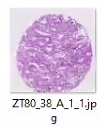
\includegraphics[width=2cm]{dataset_sample.png}
      \\
    \end{tabular}}
    \caption{Sample Dataset Image\label{figure3}}
\end{figure}

The dataset consists of 888 images, with following details. 
TMA 76 is Validation Set
TMA 80 is Test Set
TMA 111, 199 & 204 are usd as Training Set. 

    \begin{figure}[tbh]
    \centerline{\begin{tabular}{cc|c}
        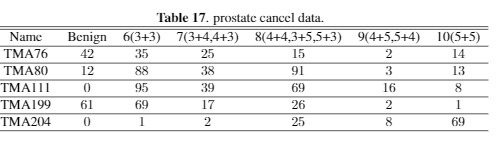
\includegraphics[width=8cm]{fig-dataset.jpeg}
      \\ 
    \end{tabular}}
    \caption{Dataset\label{figure98}}
\end{figure}

\section{Proposed system}

	Our proposed methodology for the detection of the cancerous cells involves various stages as shown in the below model. For the detection and diagnosis of cancer from microscopic biopsy images, the histopathologists normally look at the specific features in the cells and tissue structures. 
\begin{figure}[tbh]
    \centerline{\begin{tabular}{cc|c}
        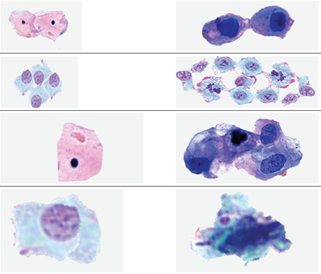
\includegraphics[width=5cm]{proposed_cancer_cell1.png}
      \\    (a)
    \end{tabular}}
    \caption{View of Normal and Cancerous cells\label{figure4}}
\end{figure}
	The various common features used for the detection and diagnosis of cancer from the microscopic biopsy images include shape and size of cells, shape and size of cell nuclei, and distribution of the cells. Our aim is to design an application which can automate the process of Cancer detection. After delving through the various methodologies and performing the comparative analysis we have finalized on the methods explained below. 
    \begin{figure}[tbh]
    \centerline{\begin{tabular}{cc|c}
        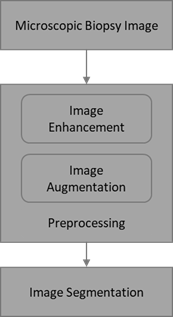
\includegraphics[width=2cm]{fig-model.png}
      \\ 
    \end{tabular}}
    \caption{Model for detection of Cancerous cells\label{figure5}}
\end{figure}

\subsection{ Preprocessing}
  
  During this stage, the microscopic images are huge in size and the samples required for the training are usually limited. Hence, we performed image enhancement and augmentation to improve the image quality required for the segmentation and for the training of the model. 
  
\textbf{\textit{ Adaptive Histogram Equalization : }}

	This methodology was used to enhance the picture quality. This approach is suitable for improving the local contrast and enhancing the definitions of edges in each region of an image.
      \begin{figure}[tbh]
    \centerline{\begin{tabular}{cc|c}
        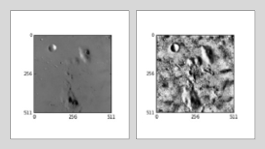
\includegraphics[width=7cm]{fig-adaptive-histogram.png}
      \\ 
    \end{tabular}}
    \caption{Comparison of the Original image and the Adaptive Histogram Equalized image\label{figure6}}
\end{figure}
  This method was chosen to enhance the image quality since is adaptive method computes several histograms, each corresponding to a distinct section of the image, and uses them to redistribute the lightness values of the image. It is therefore suitable for improving the local contrast and enhancing the definitions of edges in each region of an image.
  
  \textbf{\textit{Image Augmentation : }}}
 
	This methodology is required since we required a good amount of training data to improve the performance of the segmentation model. Hence, we had to rely upon creating training images through different ways of processing explained below. Stained colour augmentation is proven to reduce the generalization error by CNN model by simulating variations of the training data. This kind of augmentation leaves morphological features intact and focuses on simulating stain colour variations instead. 
Brightness & contrast (BC): Morphological transformations was extended by random brightness and contrast image perturbations.
Hue-Saturation-Value (HSV): This method works by randomly shifting the hue and saturation channels in the HSV colour space. This transformation produced substantially different colour distributions when applied to the training images. 
Haematoxylin-Eosin-DAB (HED): This method followed three steps as explained below:
\begin{enumerate}
\item Disentangled the haematoxylin and eosin colour channels by means of colour deconvolution using a fixed matrix. 
\item Perturb the haematoxylin and eosin stains independently. 
\item Transform the resulting stains into regular RGB colour space.
\end{enumerate}
During training, we selected the value of the augmentation hyper-parameters randomly within certain ranges to achieve stain variation. We tuned all ranges manually via visual examination. We used a scaling factor between [0.8, 1.2], elastic deformation parameters α ∈ [80, 120] and σ ∈ [9.0, 11.0], additive Gaussian noise with σ ∈ [0, 0.1], Gaussian blurring with σ ∈ [0, 0.1], brightness intensity ratio between [0.65, 1.35], and contrast intensity ratio between [0.5, 1.5].
Using HED proved to provide better performance when compared with other data augmentation techniques such as HSV, Brightness and Contrast methods. 

\subsection{Image Segmentation}

	Labelling of each pixel of an image with a corresponding class of what is being represented. So the output of segmentation is the determination of each in to a particular class. U-net is a popular CNN model that was developed for medical image segmentation, it is able to work with fewer training images to yield more precise segmentation. 
U-net architecture contains two stages. 
\begin{enumerate}
\item Contraction path /encoder: which is used to capture the context in the image. The encoder is just a traditional stack of convolutional and max pooling layers. 
\item Symmetric expanding path /decoder: which is used to enable precise localization using transposed convolutions. 
\end{enumerate}

Hence it is an end-to-end fully convolutional network, i.e. it contains Convolutional layers and does not contain any Dense layer due to which it can accept image of any size. 

      \begin{figure}[tbh]
    \centerline{\begin{tabular}{cc|c}
        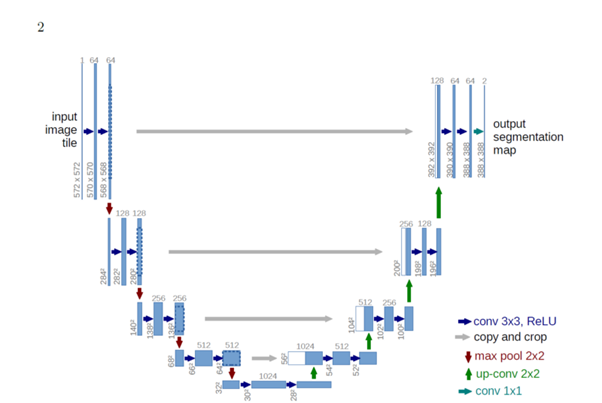
\includegraphics[width=10cm]{fig-u-net-model.png}
      \\ 
    \end{tabular}}
    \caption{U-net Architecture\label{figure7}}
\end{figure}

  We have used dice score methodology to quantify the performance of image segmentation. It is a method to evaluate the similarity between 2 sets of data, which in our case we evaluate the ground truth region with the output of the segmentation model. 
        \begin{figure}[tbh]
    \centerline{\begin{tabular}{cc|c}
        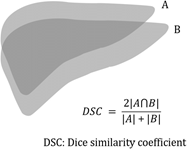
\includegraphics[width=3cm]{fig-dice.png}
      \\ 
    \end{tabular}}
    \caption{DSC Dice Similarity Coefficient\label{figure8}}
\end{figure}

A pixel can be classified as 1 or 0. If there is a mask in a pixel we state 1, if there is not a mask we state 0. Dice coefficient is a measure of overlap between two masks.1 indicates a perfect overlap while 0 indicates no overlap. For eg, lets say the ground truth is mask A, the model generated a mask B, then
\begin{itemize}
\item •	Number of positives is the total number of pixels that have intensity 1 in image A
\item •	Number of true positives is the total number of pixels which have the value 1 in both A and B. So it the intersection of the regions of ones in A and B. It is the same as using the AND operator on A and B.
\item •	Number of false positives is the number of pixels which appear as 1 in B but zero in A.
\end{itemize}

So the dice score is calculated as mentioned here, 

        \begin{figure}[tbh]
    \centerline{\begin{tabular}{cc|c}
        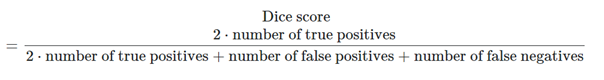
\includegraphics[width=8cm]{fig-dice-formula.png}
      \\ 
    \end{tabular}}
     \caption{Calculation\label{figure9}}
\end{figure}
  
  The Dice score is not only a measure of how many positives you find, but it also penalizes for the false positives that the method finds, like precision. The only difference is the denominator, where you have the total number of positives instead of only the positives that the method finds. So, the Dice score is also penalizing for the positives that your algorithm/method could not find. 
  
\subsection{User Interface}
    We developed a simple User Interface for Pathologists to upload the image of the cell sample , and run the model and get the 'segmentation' result. 
    
           \begin{figure}[tbh]
    \centerline{\begin{tabular}{cc|c}
        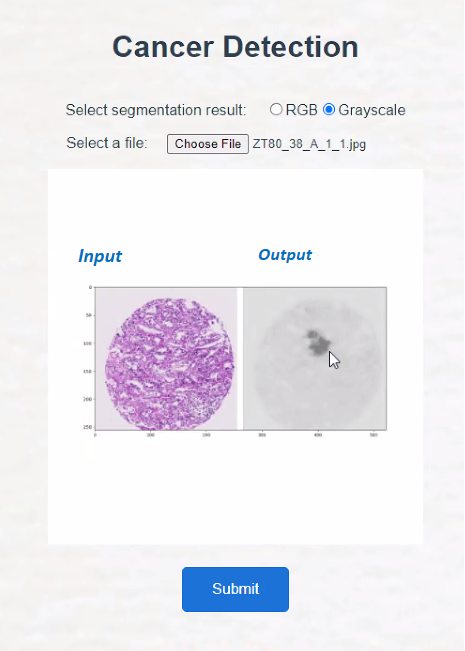
\includegraphics[width=6cm]{fig-user-interface.png}
      \\ 
    \end{tabular}}
     \caption{User Interface\label{figure97}}
\end{figure}
    
\section{Experimental results}

We evaluated various approaches and documented the quantitative and qualitative results of each approaches. 


\subsection{DeeplabV3 Model Evaluation}

We have trained \textbf{DeeplabV3 with cityscapes dataset on resnet v2}. \cite{Liang:Encoder} Following are the (hyper)parameters used and the results are below. we were not able to proceed further due to low computation power.  Find the result in Figure.
        \begin{figure}[tbh]
    \centerline{\begin{tabular}{cc|c}
       \hline\hline
    Train Epochs & 26 \\\hline
    Batch Size & 10 \\\hline
    Decay & 2e-4 \\\hline
    max iteration & 30000 \\\hline
    initial learning rate & 7e-3 \\\hline
        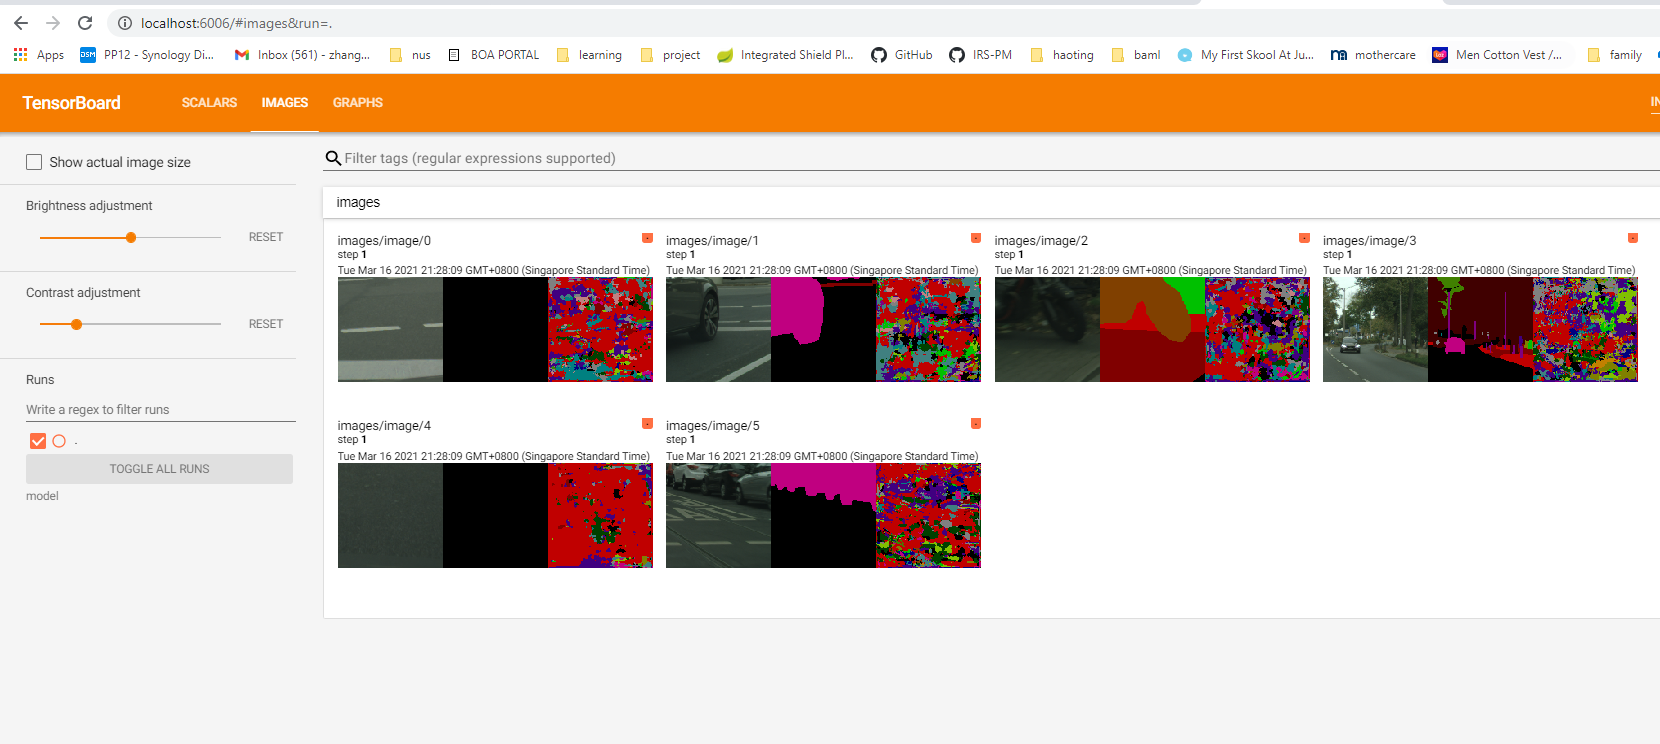
\includegraphics[width=6cm]{resnet_V2_101.png}
      \\ 
    \end{tabular}}
    \caption{DeeplabV3 on cityscapes dataset\label{figure10}}
\end{figure}

\subsection{Approach 1: Unet segmentation with MobileNetV2}
Inference speed is big concern due to low computation power, so MobileNetV2\cite{Nikhil:17UNET} has been chosen. 
Dice coefficient works well on imbalanced data, so used as loss function in Equation \ref{equation 1}
\begin{equation}\label{equation 1}
Dice Loss=1-\frac{2\sum_{pixels}(y_{true}*y_{pred})}{\sum_{pixels}(y_{true})+\sum_{pixels}(y_{pred})}
\end{equation}

Find the (hyper)parameters in table 
\begin{table}[tbh]
\caption{Approach 1 : RESULTS / OBSERVATION} \centerlin{
    \begin{tabular}{clc}
        \hline\hline
    train epochs & 36 \\\hline
    batch size & 8 \\\hline
    Learning Rate & 1e-4 \\\hline
 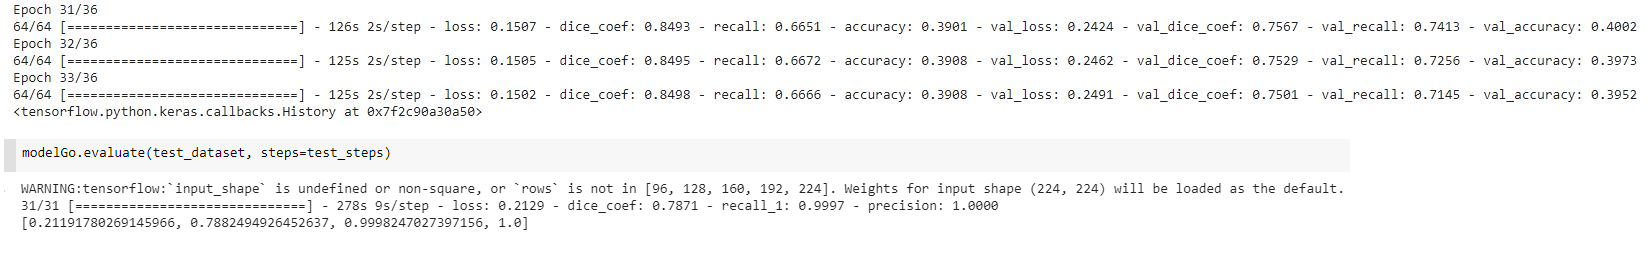
\includegraphics[width=4cm]{unet_grayscale_train_test.png}
    &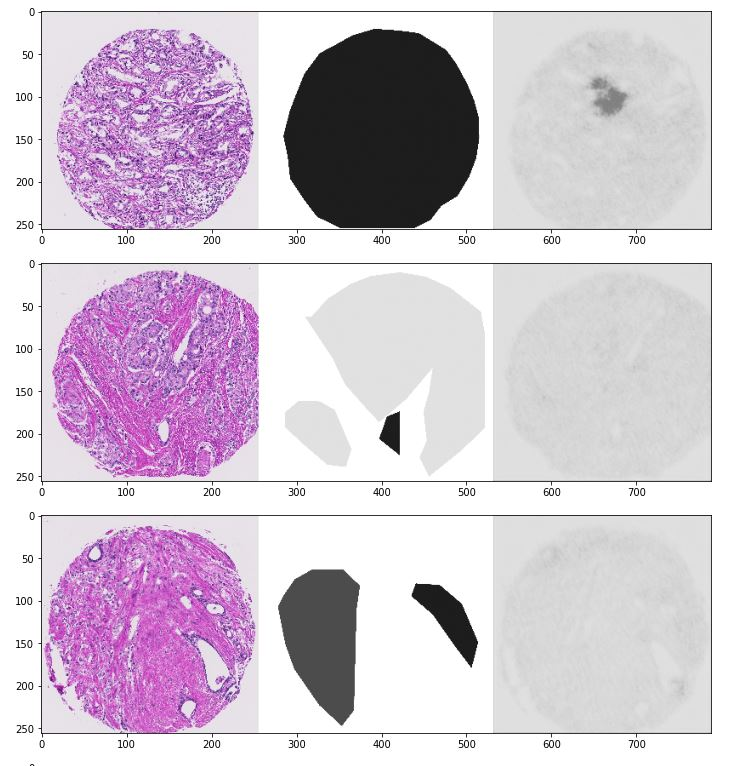
\includegraphics[width=1cm]{unet_grayscale.JPG} \\\hline\hline
\textbf{ Dice coefficient}& \textbf{\textit{$0.7871$}}\\\hline\hline
    \end{tabular}
    }
\end{table}

\subsection{Approach 2: Unet segmentation with Patch Pre-processing}
We have small dataset with\textbf{ large image size 3100*3100} and it is measure region by region as well , so created patch with \textbf{size 200*200} , the training size is increased to \textbf{73152 from 508}, so increased the batch size and reduced the epoch to speed up. we should train more, although the dice coefficient value increased but when look at some sample out, it is sparse.  We use decay to adjust learning rate after every batch update. 
Find the (hyper)parameters in table 

\begin{table}[tbh]
\caption{Approach 2 : RESULTS / OBSERVATION} \centerlin{
    \begin{tabular}{clc}
     \hline\hline
    train epochs & 16 \\\hline
    batch size & 32 \\\hline
    Learning Rate & 1e-4 \\\hline
    momentum& 0.9\\\hline
    decay&1e-4/25\\\hline
    \hline
   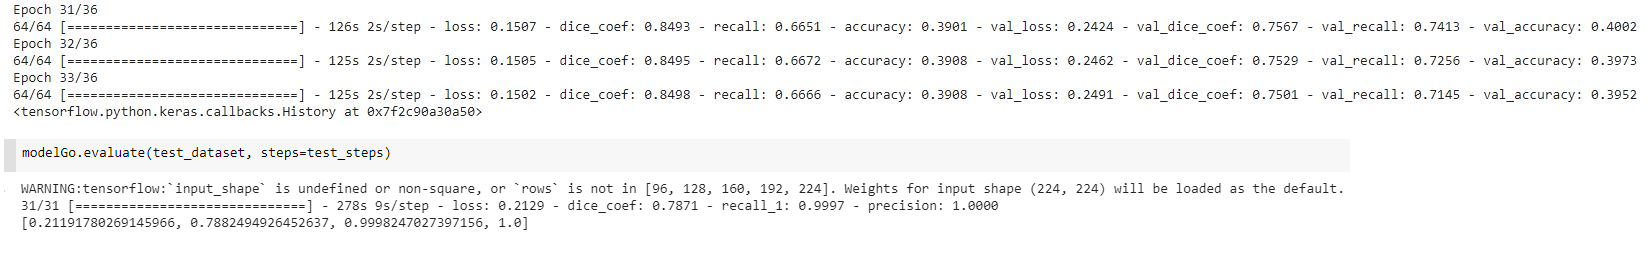
\includegraphics[width=4cm]{unet_grayscale_train_test.png}
    &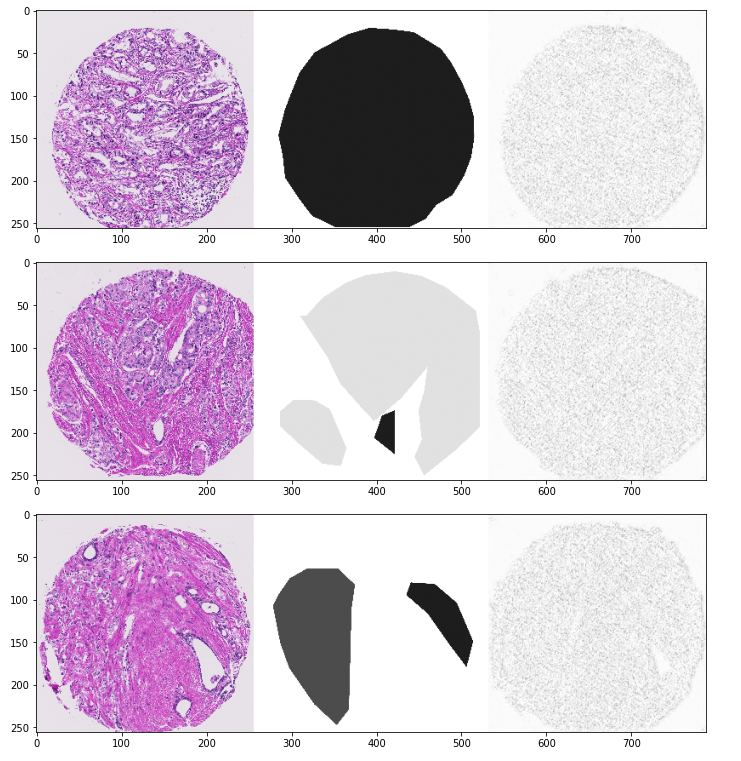
\includegraphics[width=1cm]{unet_patch.png} \\\hline\hline
\textbf{ Unet Coefficient (Approach1)}& \textbf{\textit{$0.7871$}}\\
\textbf{ Unet patch (Approach2)}& \textbf{\textit{$0.8281$}}\\\hline\hline
    \end{tabular}
    }
\end{table}

\[\]

\subsection{Approach 3: Unet segmentation by Increasing Epoch}

Following is teh setup by increasing Epoch

\begin{table}[tbh]
\caption{The (hyper)parameters}\label{table5} \centerline{
    \begin{tabular}{clc}
    \hline\hline
    train epochs & 100 \\\hline
    batch size & 8 \\\hline
    Learning Rate & 1e-4 \\\hline\hline
   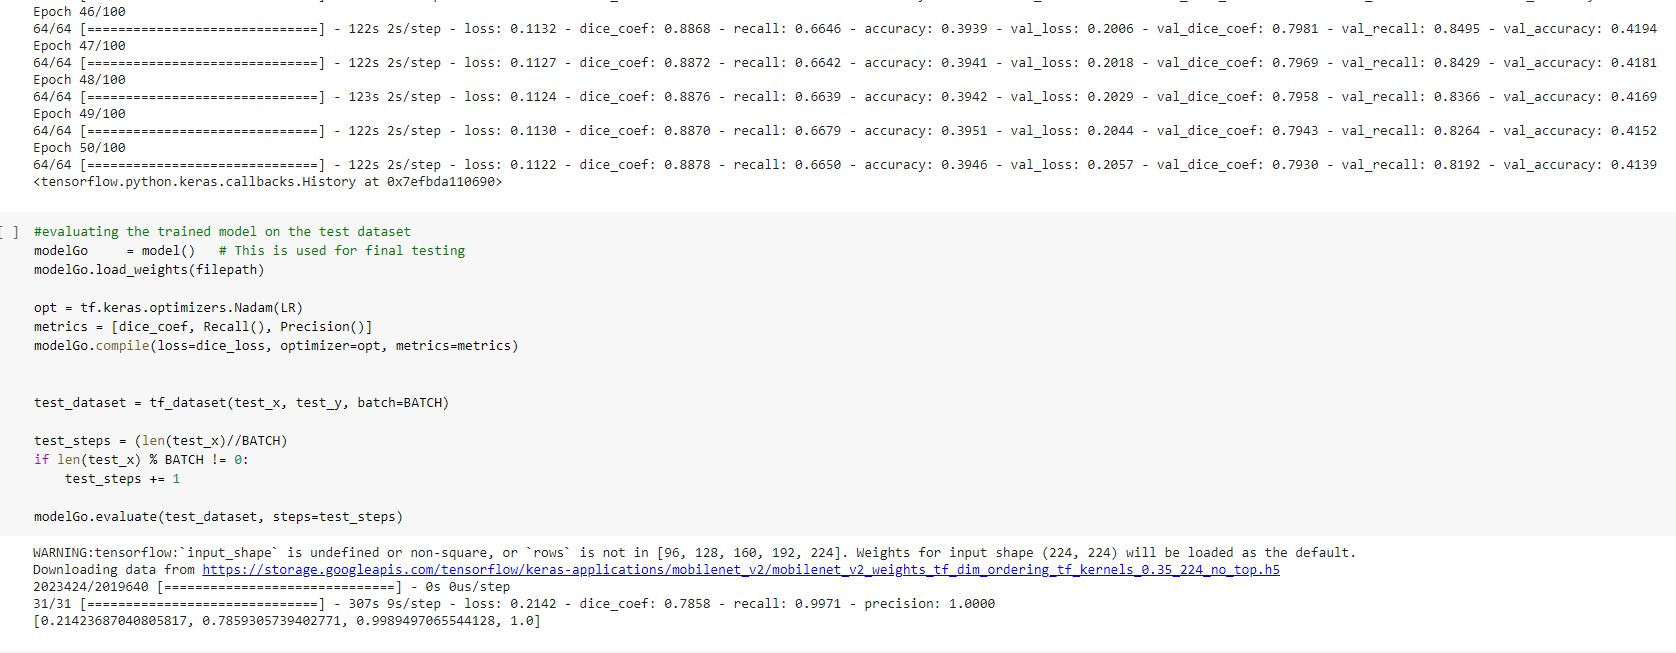
\includegraphics[width=4cm]{unet_increase_epoch_train_test.JPG}
    &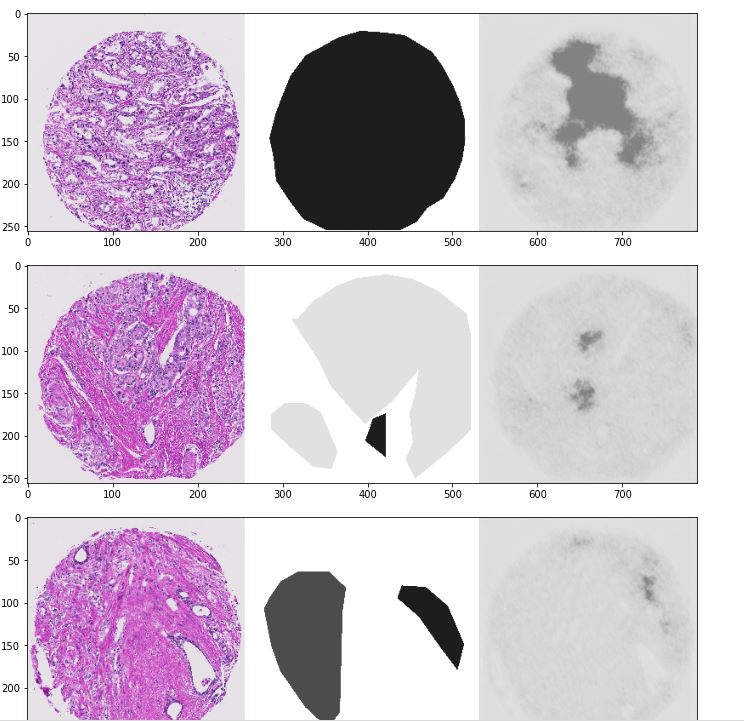
\includegraphics[width=1cm]{unet_increase_epoch.JPG} \\\hline
\textbf{ Unet Coefficient (Approach1)}& \textbf{\textit{$0.7871$}}\\
\textbf{ Unet patch (Approach2)}& \textbf{\textit{$0.8281$}}\\
\textbf{ Unet increased epoch (Approach3)}& \textbf{\textit{$0.7858$}}\\\hline\hline
    \end{tabular}
    }
\end{table}

\subsection{Approach 4: Unet segmentation with HSV augmentation}
1 HSV color space \cite{David:20Quantifying} augmented image is generated from each original image, trained on top of pre-trained unet model in Approach 1 and HSV augmentation function is provided below , subscript i represents hue or saturation channel, \alpha is drawn from a uniform distribution [-1,1] \cite{Fuentes:Spectral}


\begin{equation}\label{equation 2}
S'_{i}=\alpha_{i}S_{i} 
\end{equation}
The reasons as for why our model was unable to fully segment the epidermal area in these images, varies from image to image. One image has a piece of folded tissue in the epidermis area, which our system didn’t recognize. Another image comprise of an epidermis broken up into several parts, where some of these were deemed as too small and removed in the post-processing stage. 

\begin{table}[tbh]
\caption{The (hyper)parameters}\label{table6} \centerline{
    \begin{tabular}{clc}
    \hline\hline
    train epochs & 36 \\
    batch size & 8 \\
    Learning Rate & 1e-4 \\\hline\hline
   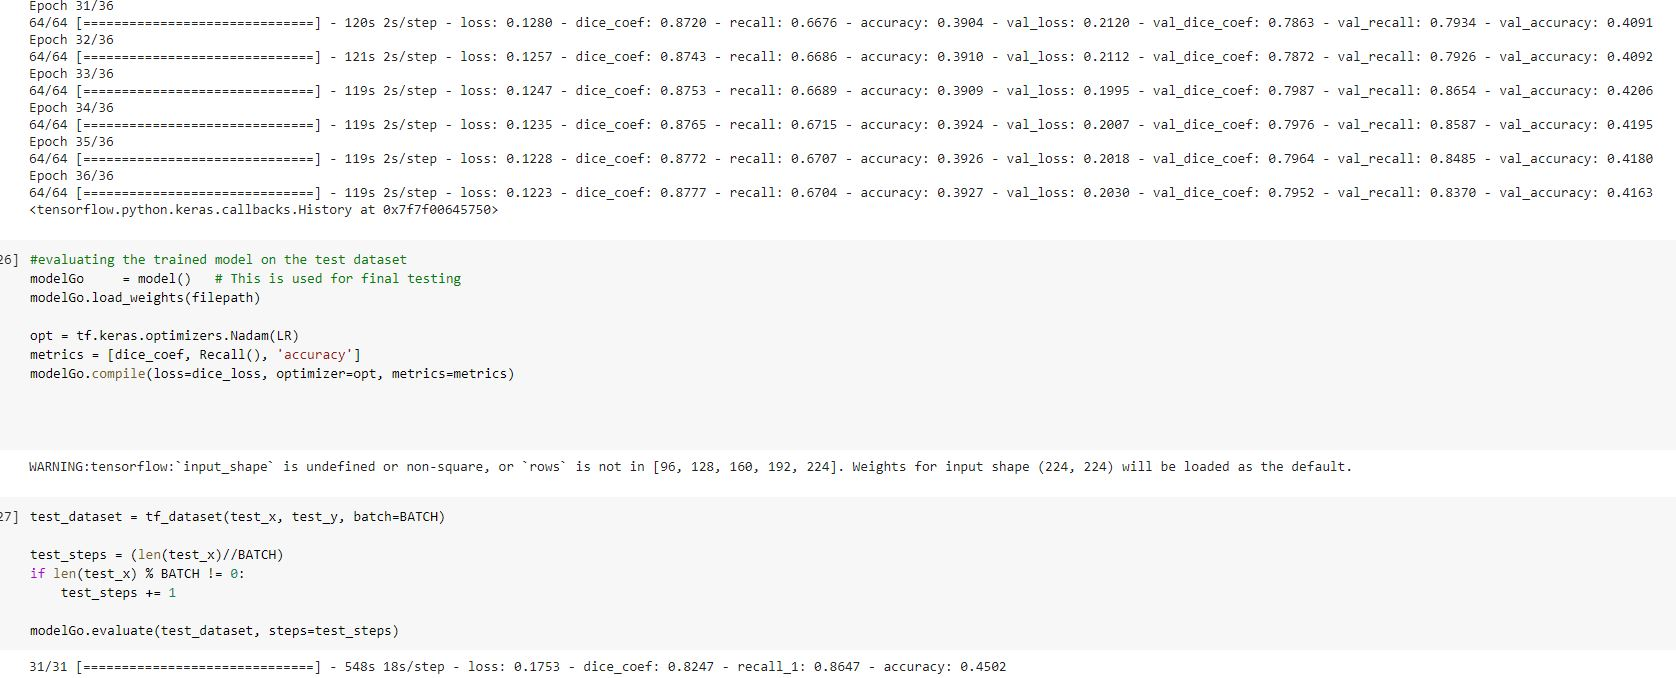
\includegraphics[width=3cm]{unet_hsv_train_test.JPG}
    &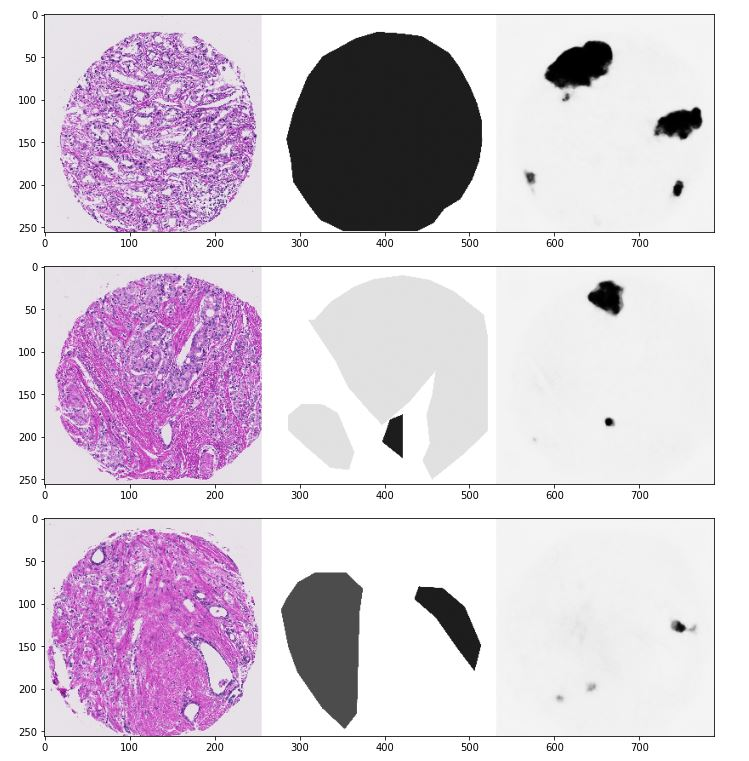
\includegraphics[width=1cm]{unet_hsv.JPG} \\\hline
\textbf{ Unet Coefficient (Approach1)}& \textbf{\textit{$0.7871$}}\\
\textbf{ Unet patch (Approach2)}& \textbf{\textit{$0.8281$}}\\
\textbf{ Unet increased epoch (Approach3)}& \textbf{\textit{$0.7858$}}\\
\textbf{ Unet with HSV augmentation (Approach4)}& \textbf{\textit{$0.8247$}}\\\hline\hline
    \end{tabular}
    }
\end{table}

\subsection{Approach 5: Unet segmentation with HED augmentation}
3 HED augmented images are generated from each original image, the training size is increased to 1289 from 508 and HED augmentation function is provided below in Equation, \textbf{i} represents each stain channel, alpha is drawn from a uniform distribution U(1 − alpha; 1 + alpha),beta is drawn from a uniform distribution U(−alpha; alpha), and typically alpha = 0.05 \cite{Tellez:Whole}
\begin{equation}\label{equation 3}
S'_{i}=\alpha_{i}S_{i}+\beta_{i} 
\end{equation}
\begin{table}[tbh]
\caption{The (hyper)parameters}\label{table6} \centerline{
    \begin{tabular}{clc}
    \hline\hline
    train epochs & 36 \\
    batch size & 8 \\
    Learning Rate & 1e-4 \\\hline\hline
   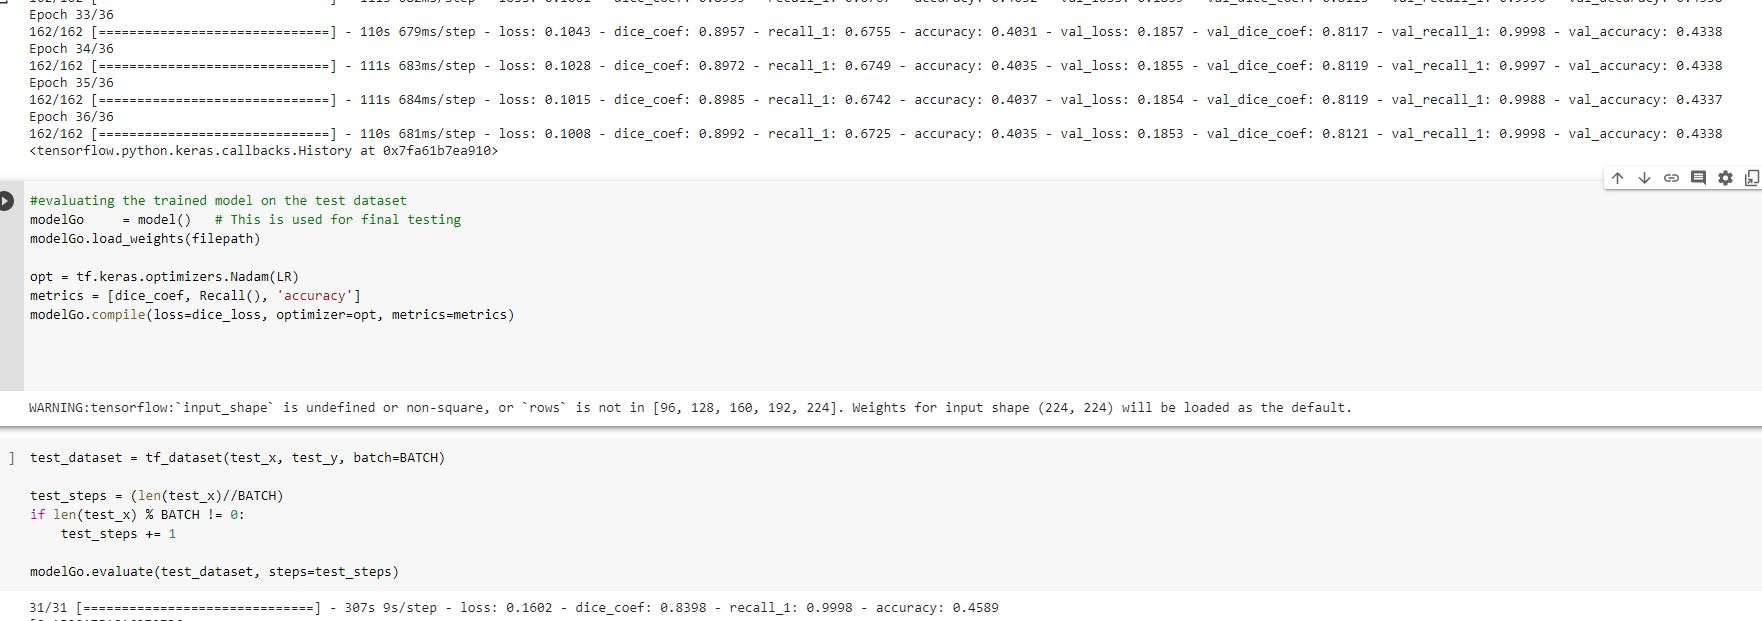
\includegraphics[width=4cm]{unet_hed_train_test.JPG}
    &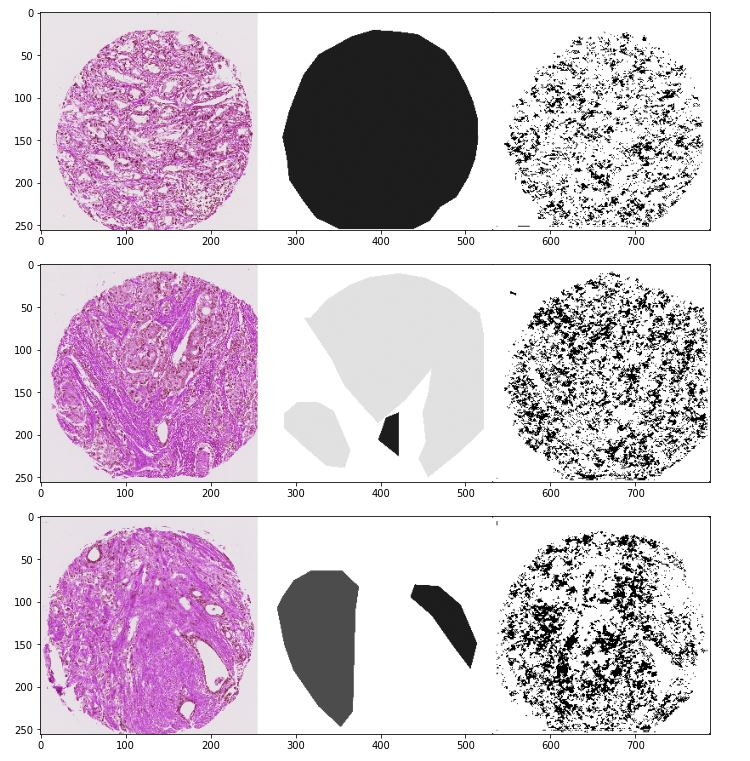
\includegraphics[width=2cm]{unet_hed.JPG} \\\hline
\textbf{ Unet Coefficient (Approach1)}& \textbf{\textit{$0.7871$}}\\
\textbf{ Unet patch (Approach2)}& \textbf{\textit{$0.8281$}}\\
\textbf{ Unet increased epoch (Approach3)}& \textbf{\textit{$0.7858$}}\\
\textbf{ Unet HSV (Approach4)}& \textbf{\textit{$0.8247$}}\\
\textbf{ Unet HED  (Approach5)}& \textbf{\textit{$0.8398$}}\\\hline\hline
    \end{tabular}
    }
\end{table}

The result clearly shows that HSV and HED did not make any difference in teh efficiency. 

This would potentially be a limitation with the data set being used. 

\subsection{Approach 6: Unet multi-class segmentation }
Try Multidimensional Dice coefficient since we have RGB masks 
Multidimensional Dice coefficient \cite{Sohini:Multi-class} is used as loss function and is provided in Figure \ref{figure7} 
\begin{figure}[tbh]
    \centerline{\begin{tabular}{c}
        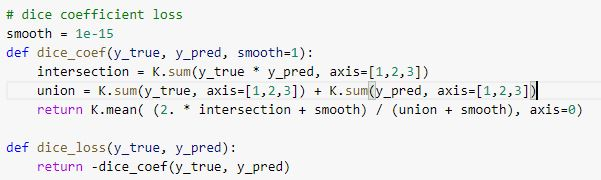
\includegraphics[width=8cm,height=3cm]{multidimensional-dice.JPG}
    \end{tabular}}
    \caption{Unet multi-class segmentation \label{figure7}}
\end{figure}
The evaluation & results shows greater efficiency. 

   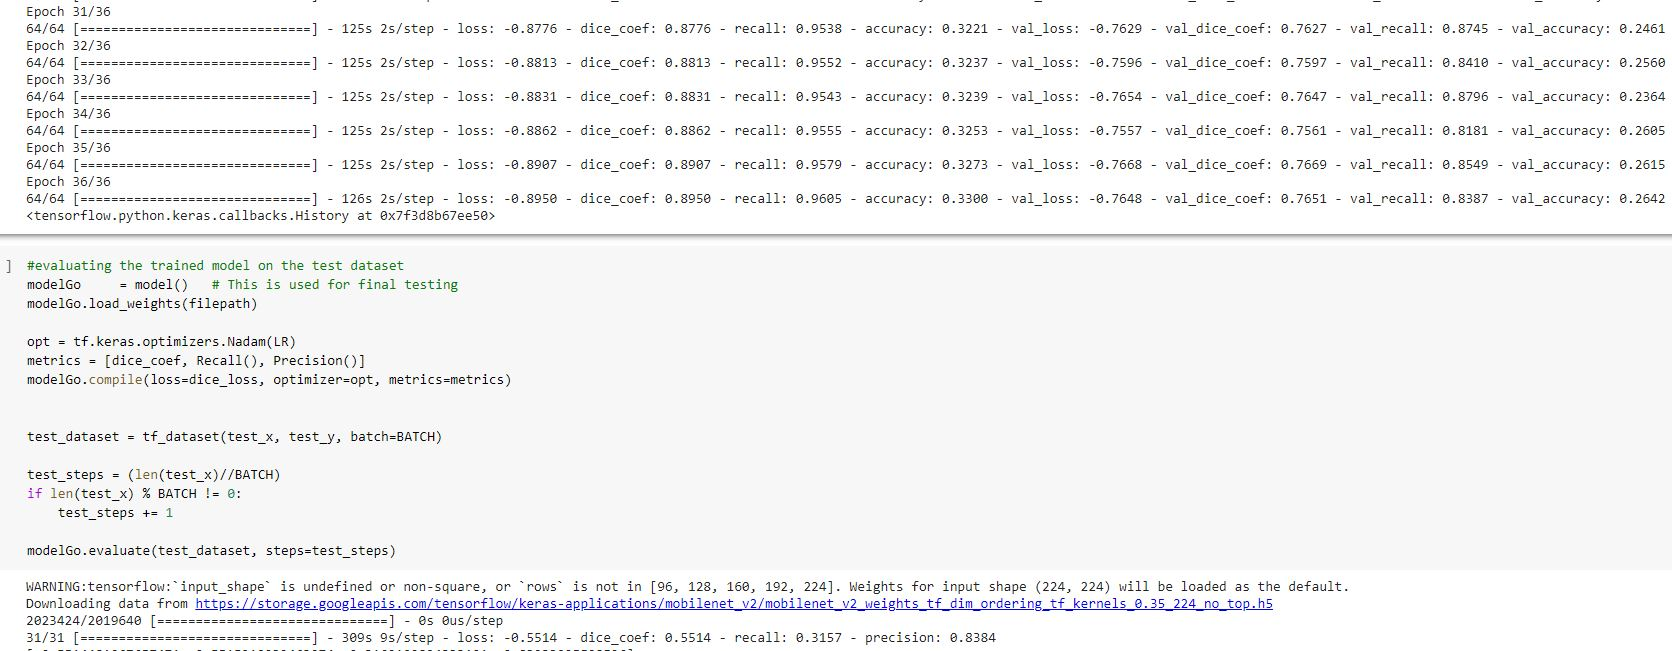
\includegraphics[width=3cm]{unet_color_train_test.JPG}
    &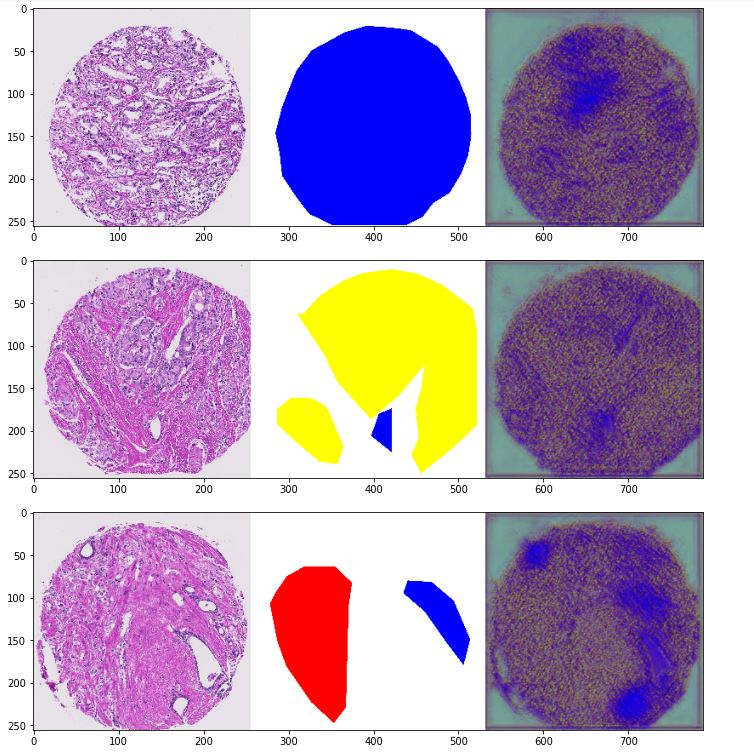
\includegraphics[width=1cm]{unet_color.JPG} \\
    
\begin{table}[tbh]
\caption{The (hyper)parameters}\label{table6} \centerline{
    \begin{tabular}{clc}
    \hline\hline
    train epochs & 36 \\
    batch size & 8 \\
    Learning Rate & 1e-4 \\\hline
\textbf{ Unet Coefficient (Approach1)}& \textbf{\textit{$0.7871$}}\\
\textbf{ Unet patch (Approach2)}& \textbf{\textit{$0.8281$}}\\
\textbf{ Unet increased epoch (Approach3)}& \textbf{\textit{$0.7858$}}\\
\textbf{ Unet HSV (Approach4)}& \textbf{\textit{$0.8247$}}\\
\textbf{ Unet HED  (Approach5)}& \textbf{\textit{$0.8398$}}\\
\textbf{ Unet multi-class segmentation (Approach 6)}& \textbf{\textit{$0.5514$}}\\
\hline\hline
    \end{tabular}
    }
\end{table}

\subsection{Approach 7: Unet multi-class HSV }
try multi-class segmentation with HSV augmented data on top of pre-trained multi-class segmentation in Approach 6.
The evaluation & results shows greater efficiency. 

Following is the result (segmended) image. 

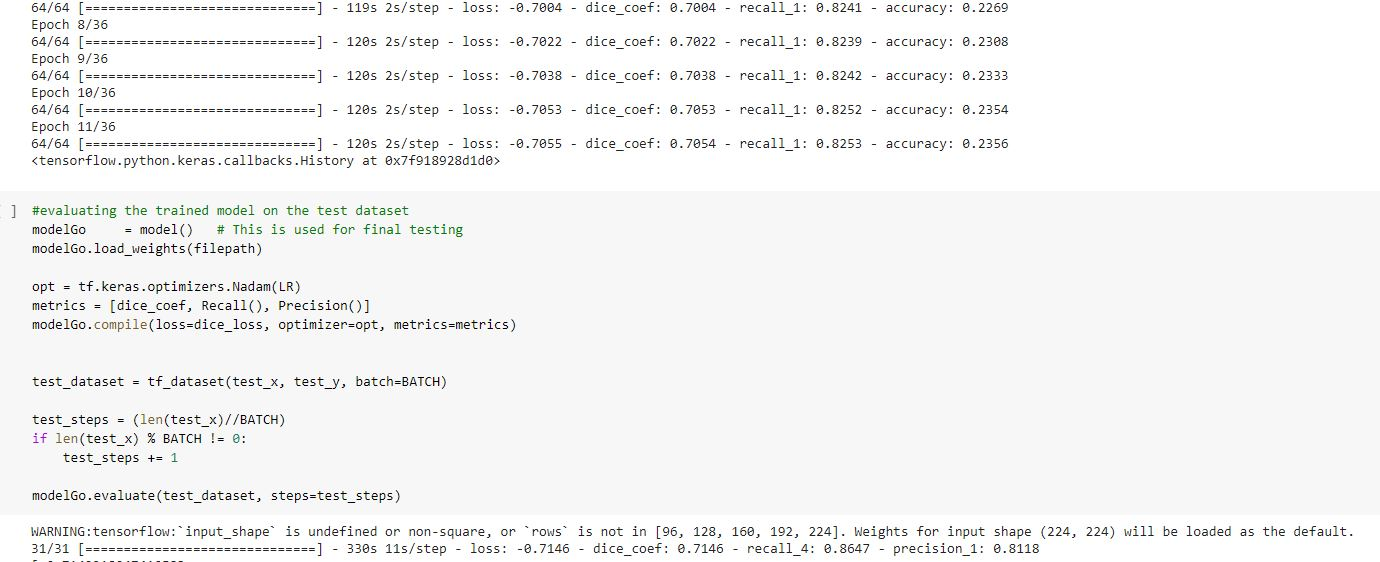
\includegraphics[width=3cm]{unet_color_hsv_train_test.JPG}
    &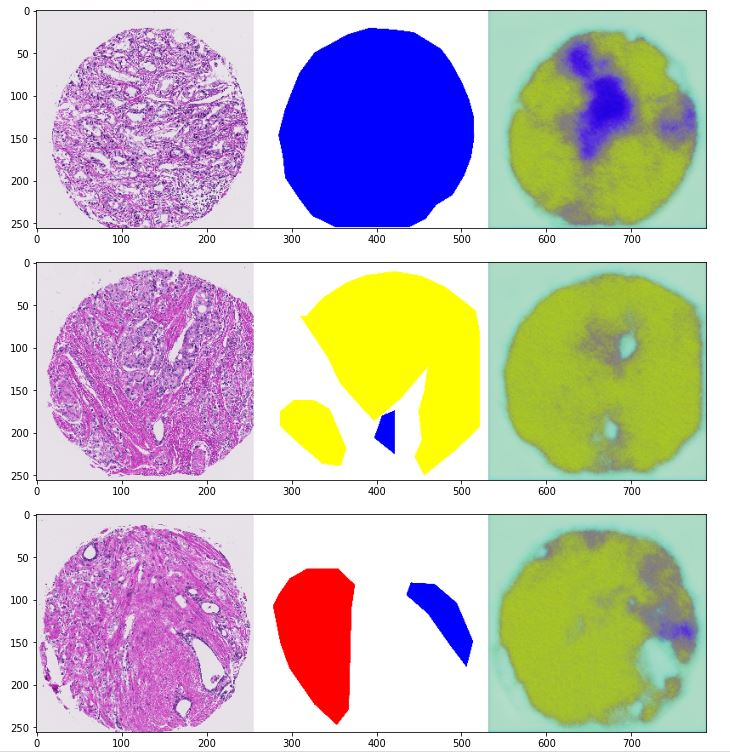
\includegraphics[width=2cm]{unet_color_hsv.JPG} \\
    
\begin{table}[tbh]
\caption{The (hyper)parameters}\label{table6} \centerline{
    \begin{tabular}{clc}
    \hline\hline
    train epochs & 36 \\
    batch size & 8 \\
    Learning Rate & 1e-4 \\\hline\hline
\textbf{ Unet Coefficient (Approach1)}& \textbf{\textit{$0.7871$}}\\
\textbf{ Unet patch (Approach2)}& \textbf{\textit{$0.8281$}}\\
\textbf{ Unet increased epoch (Approach3)}& \textbf{\textit{$0.7858$}}\\
\textbf{ Unet HSV (Approach4)}& \textbf{\textit{$0.8247$}}\\
\textbf{ Unet HED  (Approach5)}& \textbf{\textit{$0.8398$}}\\
\textbf{ Unet multi-class segmentation (Approach 6)}& \textbf{\textit{$0.5514$}}\\
\textbf{Unet multi-class HSV (Approach 7)}& \textbf{\textit{$0.7146$}}\\
\hline\hline
    \end{tabular}
    }
\end{table}



\subsection{Approach 8: Unet multi-class HED }
Try multi-class segmentation with HED augmented data

    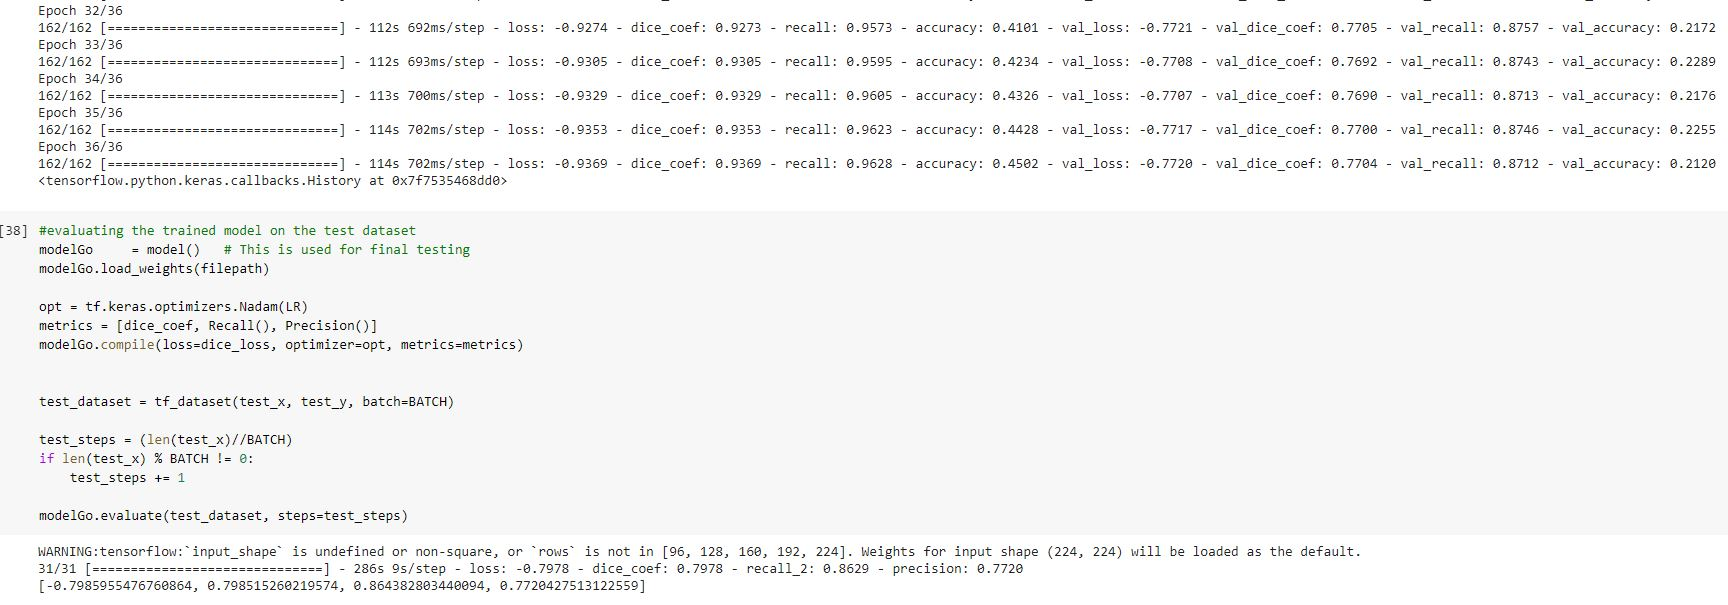
\includegraphics[width=3cm]{unet_color_hed_train_test.JPG}
    &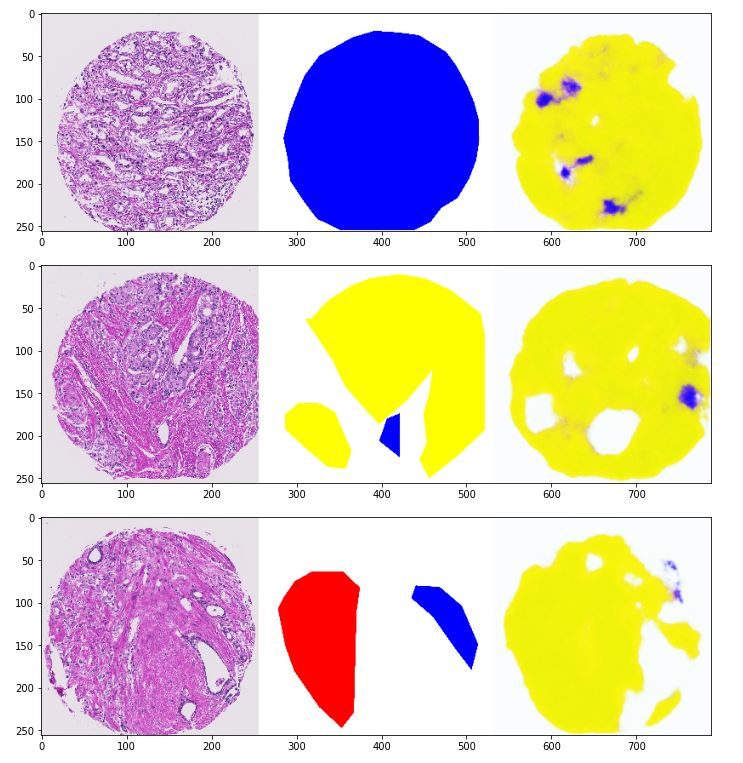
\includegraphics[width=3cm]{unet_color_hed.JPG} \\
    
\begin{table}[tbh]
\caption{The (hyper)parameters}\label{table6} \centerline{
    \begin{tabular}{clc}
    \hline\hline
    train epochs & 36 \\
    batch size & 8 \\
    Learning Rate & 1e-4 \\\hline

\textbf{ Unet Coefficient (Approach1)}& \textbf{\textit{$0.7871$}}\\
\textbf{ Unet patch (Approach2)}& \textbf{\textit{$0.8281$}}\\
\textbf{ Unet increased epoch (Approach3)}& \textbf{\textit{$0.7858$}}\\
\textbf{ Unet HSV (Approach4)}& \textbf{\textit{$0.8247$}}\\
\textbf{ Unet HED  (Approach5)}& \textbf{\textit{$0.8398$}}\\
\textbf{ Unet multi-class segmentation (Approach 6)}& \textbf{\textit{$0.5514$}}\\
\textbf{Unet multi-class HSV (Approach 7)}& \textbf{\textit{$0.7146$}}\\
\textbf{Unet multi-class HED (Approach 8)}& \textbf{\textit{$0.7978$}}\\
\hline\hline
    \end{tabular}
    }
\end{table}
\section{Conclusions and future work}

\subsection{Conclusion}

	Our team had a great time working on this project, and we definitely picked up some useful skills along the way. 

	The problem statement is to show the cancerous / non-cancerous cell segmentation as soon as possible, to the pathologist as a recommendation. With multiple segmentation approaches we tried in this practice module, we conclude the following. 
\begin{enumerate}
\item Approach 2 (Unet Patch), Approcah 4 (HSV) and Approach 5 (HED) are more than 80\% accuracy. Color space augmentation (HSV or HED) can help increase the accuracy. 
\item Classical Dice Coefficient Loss function is efficient (approach 1, 2,3,4 & 5) and have more accuracy than Multi-dimensional Dice Coefficient function (approach 6, 7 and 8). 
\item Patch Processing with half of the epoh (epoh=16) can reach the higher accuracy than Prcessing without Patching (epoh =36), or patch processing with Higher Epoh (epoh-36).   
\item More epoh does not mean higher accuracy.  For eg., Approach 3 (epoh=100) is not having good accuracy than Approach 1 (epoh=36)
\end{enumerate}

\subsection{Future Work}
\begin{enumerate}
\item More analysis can be done with combining multiple approaches to increase the accuracy of the model and we could use Otsu’s threshold in Figure \ref{figure8} to mask off some artifacts/imperfection in H&E stained images. \cite{David:21Quantifying}
in Figure  
\begin{figure}[tbh]
    \centerline{\begin{tabular}{c}
        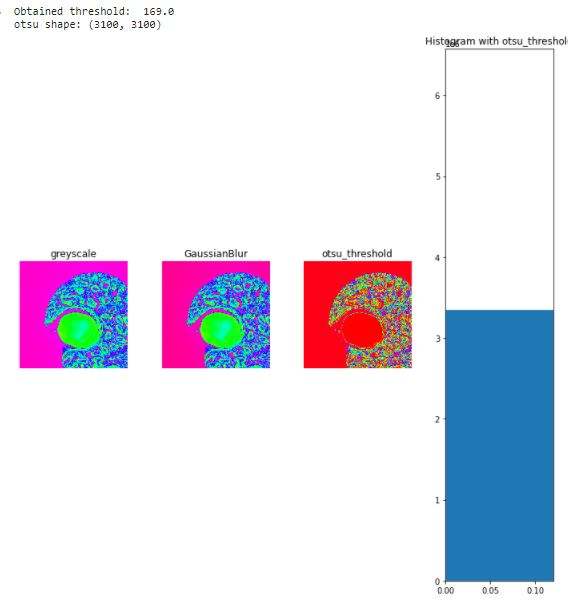
\includegraphics[width=5cm,height=3cm]{ostu.JPG}
    \end{tabular}}
    \caption{otsu threshold \label{figure8}}
\end{figure}

\item Classification: Classification of the segmented image, can help to arrive an accurate recommendation to pathologist. 
\item Use more geographical specific Private data-set to create and train the models to increase the usage of the model for specific institution (like major hospital). 

\section{Contributions}
\subsection{Zhang Yu - A0213498X}
\textbf{Development, Integration, Training \& Documentation : } Research \& understanding of the domain,  Data-set Identification, Selection, and understanding. Technical Design. UI and model development , training \& testing.Documentation \& presentation \& .

\subsection{Natarajan Anandan - A0213514U }
\textbf{ Project Managmeent, Busienss Analysis \& Domain Analysis,  Documentation \& Presentations}: Project Management, Research \& understanding of the domain, Study the previous research and models already in the Technology area for this domain, UI Design \& Testing. Documentation \& presentation. Initial proposal, mid project presentation and final project documentation.
\end{enumerate}
 		   
\bibliographystyle{IEEEbib}
\bibliography{references}
\end{document}
